% Template for PLoS
% Version 3.3 June 2016
%
% % % % % % % % % % % % % % % % % % % % % %
%
% -- IMPORTANT NOTE
%
% This template contains comments intended 
% to minimize problems and delays during our production 
% process. Please follow the template instructions
% whenever possible.
%
% % % % % % % % % % % % % % % % % % % % % % % %

% Created to hold supplementary information

\documentclass[10pt,letterpaper]{article}

\usepackage[top=0.85in,left=2in,footskip=0.75in]{geometry}

% amsmath and amssymb packages, useful for mathematical formulas and symbols
\usepackage{amsmath,amssymb}

% Use adjustwidth environment to exceed column width (see example table in text)
\usepackage{changepage}

% Use Unicode characters when possible
\usepackage[utf8x]{inputenc}

% textcomp package and marvosym package for additional characters
\usepackage{textcomp,marvosym}

% cite package, to clean up citations in the main text. Do not remove.
\usepackage{cite}

% Use nameref to cite supporting information files (see Supporting Information section for more info)
\usepackage{nameref,hyperref}

% line numbers
\usepackage[right]{lineno}

% ligatures disabled
\usepackage{microtype}
\DisableLigatures[f]{encoding = *, family = * }

% color can be used to apply background shading to table cells only
\usepackage[table]{xcolor}

% array package and thick rules for tables
\usepackage{array}

% create "+" rule type for thick vertical lines
\newcolumntype{+}{!{\vrule width 2pt}}

% added by George
%\usepackage{wrapfig}
%\usepackage{caption}
\usepackage{subcaption}

% create \thickline for thick horizontal lines of variable length
\newlength\savedwidth
\newcommand\thickcline[1]{%
  \noalign{\global\savedwidth\arrayrulewidth\global\arrayrulewidth 2pt}%
  \cline{#1}%
  \noalign{\vskip\arrayrulewidth}%
  \noalign{\global\arrayrulewidth\savedwidth}%
}

% \thickhline command for thick horizontal lines that span the table
\newcommand\thickhline{\noalign{\global\savedwidth\arrayrulewidth\global\arrayrulewidth 2pt}%
\hline
\noalign{\global\arrayrulewidth\savedwidth}}


% Remove comment for double spacing
%\usepackage{setspace} 
%\doublespacing

% Text layout
\raggedright
\setlength{\parindent}{0.5cm}
\textwidth 5.25in 
\textheight 8.75in

% Bold the 'Figure #' in the caption and separate it from the title/caption with a period
% Captions will be left justified
\usepackage[aboveskip=1pt,labelfont=bf,labelsep=period,justification=raggedright,singlelinecheck=off]{caption}
\renewcommand{\figurename}{Fig}


% Remove brackets from numbering in List of References
\makeatletter
\renewcommand{\@biblabel}[1]{\quad#1.}
\makeatother

% Leave date blank
\date{}

% Header and Footer with logo
\usepackage{lastpage,fancyhdr,graphicx}
\usepackage{epstopdf}
\pagestyle{myheadings}
\pagestyle{fancy}
\fancyhf{}
\setlength{\headheight}{27.023pt}
\lhead{
\includegraphics[width=3.0in]{PLOS-submission.eps}}
\rfoot{\thepage/\pageref{LastPage}}
\renewcommand{\footrule}{\hrule height 2pt \vspace{2mm}}
\fancyheadoffset[L]{1.25in}
\fancyfootoffset[L]{1.25in}
\lfoot{\sf PLOS}

%% Include all macros below

\newcommand{\lorem}{{\bf LOREM}}
\newcommand{\ipsum}{{\bf IPSUM}}

%% END MACROS SECTION

\begin{document}



\vspace{30mm}

\begin{table}[!ht]
%\begin{adjustwidth}{-0.5in}{0in} % Comment out/remove adjustwidth environment if table fits in text column.
\centering
\scalebox{0.9}{
\begin{tabular}{|l+l|l|l|l|l|l|l|}
\hline
%\multicolumn{4}{|l|}{\bf Heading1} & \multicolumn{4}{|l|}{\bf Heading2}\\ \thickhline
Therapeutic & FDA Approval Date & Unique Identifier & US Patent & Publication Date  \\ \hline
$Alemtuzumab$ & May 2001 & BLA: 103948 & US5846534 & Dec 1998\\ \hline
$Imatinib$ & May 2001 & NDA: 021335 & US5521184 &  May 1996 \\ \hline
$Nelarabine$ & Oct 2005 & NDA: 021877 & US5424295 & Jun 1995  \\ \hline
$Ramucirumab$ & Apr 2014 & BLA: 125477 & US7498414 & Mar 2009  \\ \hline
$Sunitinib$ & Jan 2006  & NDA: 021938  & US6573293 & Jun 2003 \\ \hline
\end{tabular}}
\vspace{2 mm}
\caption{
{\bf Case Studies of Five Anti-Cancer Agents} Five anti-cancer therapeutics, with FDA approval dates ranging from 2001 to 2014, were selected as case studies. The active ingredient for each of these five therapeutics is listed in column 1. The unique identifier for each therapeutic is the FDA assigned NDA or BLA number. While multiple patents are typically associated with a drug or biological, the single US patent number displayed represents the primary invention that preceded approval of the therapeutic. The publication date for each patent is listed in the last column.}
%\begin{flushleft}  
%\end{flushleft}
\label{table1}
%\end{adjustwidth}
\end{table}
\clearpage


\begin{table}[!ht]
%\begin{adjustwidth}{-0.5in}{0in} % Comment out/remove adjustwidth environment if table fits in text column.
\centering
\scalebox{0.9}{
\begin{tabular}{|l+l|l|l|l|l|l|l|}
\hline
%\multicolumn{4}{|l|}{\bf Heading1} & \multicolumn{4}{|l|}{\bf Heading2}\\ \thickhline
Therapeutic & citing\_pmid count & citing\_sid count & cited\_sid count  & cited\_pmid count  \\ \hline
$Alemtuzumab$ & 599 & 587 (1\%) & 8840 (2\%) & 7071(20\%)\\ \hline
$Imatinib$ & 1380 & 1373(1\%) & 27326(1\%) &  23340(17\%) \\ \hline
$Nelarabine$ & 104 & 104(0\%) & 2476(1\%) & 1990(20\%)  \\ \hline
$Ramucirumab$ & 1820 & 1804(1\%) & 48587(0\%) & 40973(19\%)  \\ \hline
$Sunitinib$ & 1512  & 1509(0\%)  & 33895(0\%) & 28661(15\%) \\ \hline
\end{tabular}
}
\vspace{2.5 mm}
\caption{{\bf Citation Counts and Mapping Between Bibliographic Databases} Five anti-cancer therapeutics were selected as case studies. A foundational set of references (citing\_pmid) was assembled for each therapeutic from patents, clinical trials, regulatory documents, and the scientific literature (Materials and Methods). Citing\_pmids were mapped to Scopus identifiers (citing\_sid), which were used, in turn, to retrieve cited publications (cited\_sid). Cited\_sids were mapped back to PubMed identifiers (cited\_pmid).The number of  identifiers at each stage of the mapping process is shown along with percentage loss (in parentheses) when mapping across PubMed and Scopus or due to null values in the cited\_sid field} 
\label{table2}
%\end{adjustwidth}
\end{table}
\clearpage

\begin{table}[!ht]
\begin{adjustwidth}{-1.0in}{0in} % Comment out/remove adjustwidth environment if table fits in text column.
\centering
\scalebox{0.8}{\begin{tabular}{|l+l|l|l|l|l|l|l|}
\hline
%\multicolumn{4}{|l|}{\bf Heading1} & \multicolumn{4}{|l|}{\bf Heading2}\\ \thickhline
\hline
SourceYear & SourceName & Author(s) \\ 
  \hline
1958 & J. Am. Stat. Assoc. & Kaplan E.R., Meier P. \\ 
1963 & Science & Jerne, N. K. and Nordin, A. A.  \\ 
1972 & J R Stat Soc & Cox DR.  \\ 
1976 & Anal. Biochem. & Bradford MM \\ 
1977 & Br J Cancer & R. Peto, M.C. Pike, and P. Armitage  \\ 
1977 & Proc. Natl. Acad. Sci. & Sanger, F., S. Nicklen, and A.R. Coulson.  \\ 
1983 & J Immunol Methods & Mosmann T  \\ 
1984 & Adv Enzyme Regul & T.C. Chou, and P. Talalay  \\ 
1989 & Molecular Cloning: A Laboratory Manual & Sambrook, J., Fritsch, E. and Maniatis, T.  \\ 
1994 & Acta Crystallogr D & Collaborative Computational Project 4 \\ 
1994 & Acta Crystallogr. A & Navaza J.  \\ 
1997 & Cell & Levine, A. J. \\ 
1997 & Am. J. Pathol. & Perez-Atayde, A. R., Sallan, S. E., Tedrow, U., Connors, S., Allred, E., and Folkman, J.  \\ 
1998 & CA: A Cancer Journal for Clinicians & SH Landis T Murray S Bolden PA Wingo \\ 
\hline
\end{tabular}}
\vspace{2.5 mm}
\caption{{\bf Intersection of Five Networks: Second Generation Publications} Publications common to all networks at the second generation level (cited\_sid, Fig 2). } 
\label{table3}
\end{adjustwidth}
\end{table}
\clearpage

\begin{figure}[!h]
\centering
\begin{subfigure}{.5\textwidth}
  \centering
  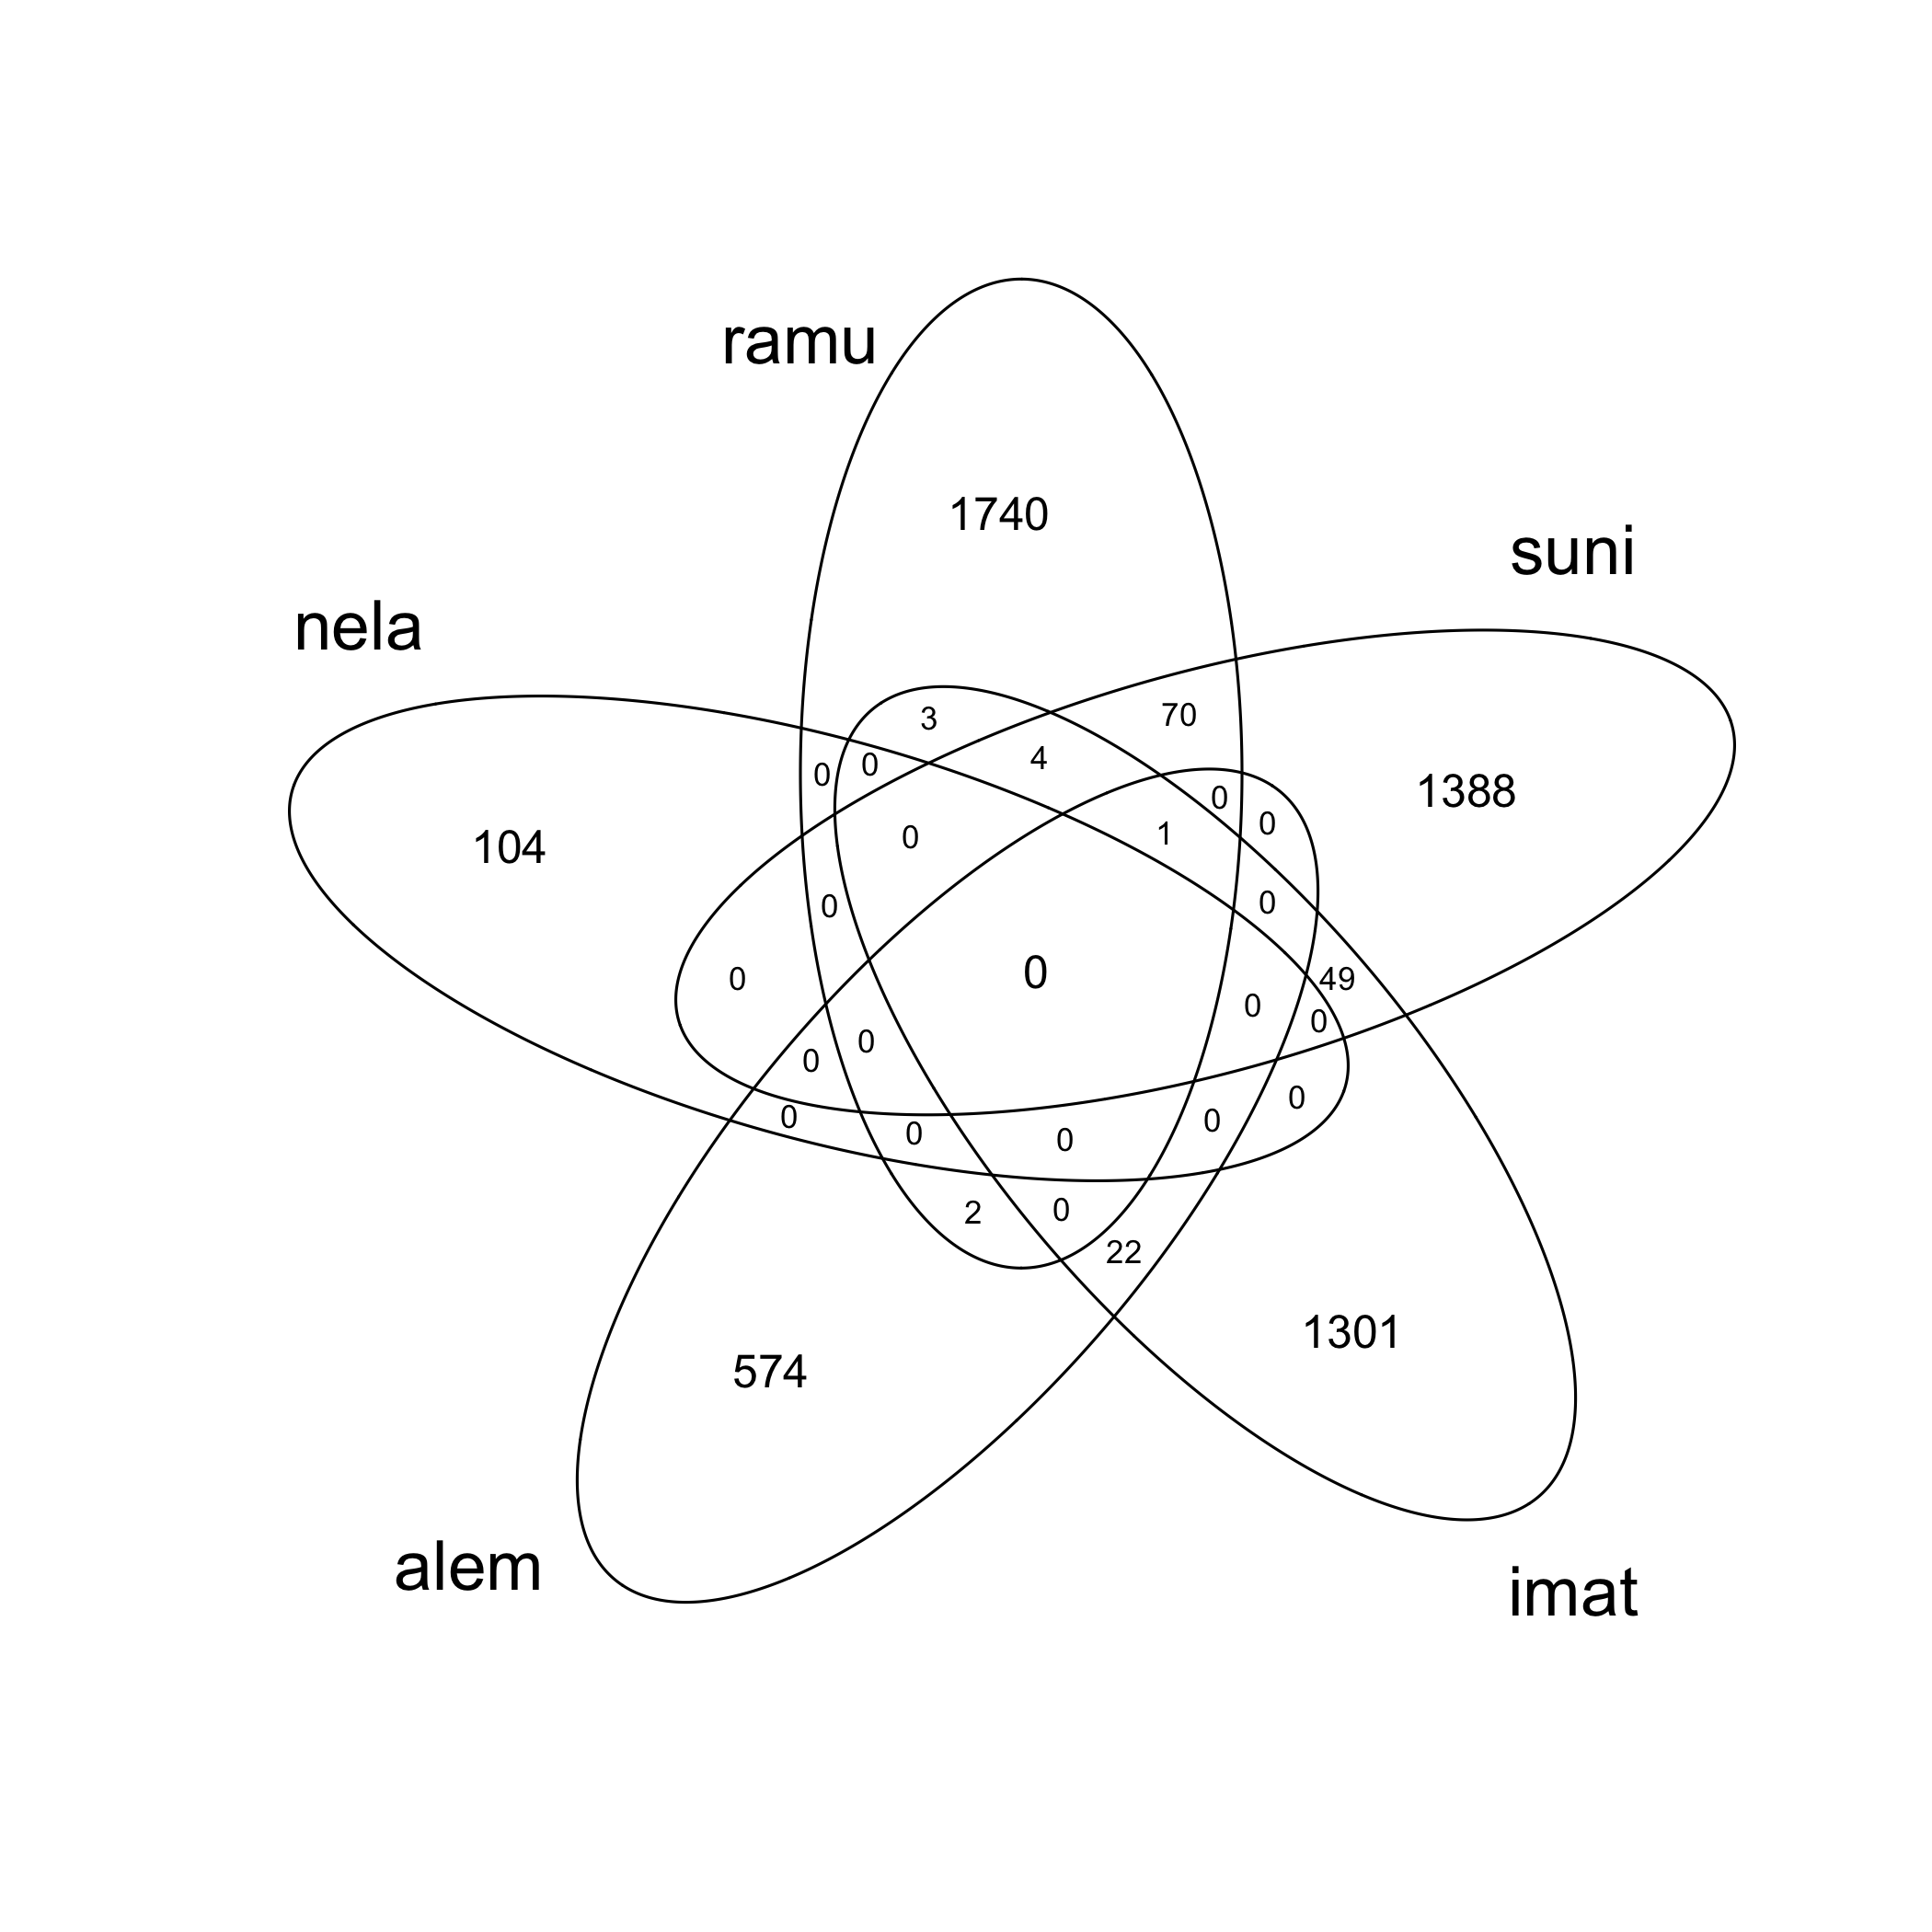
\includegraphics[width=.95\linewidth]{citing_pmid.png}
  %\caption{}
  \label{fig:sub1}
\end{subfigure}%
\begin{subfigure}{.5\textwidth}
  \centering
  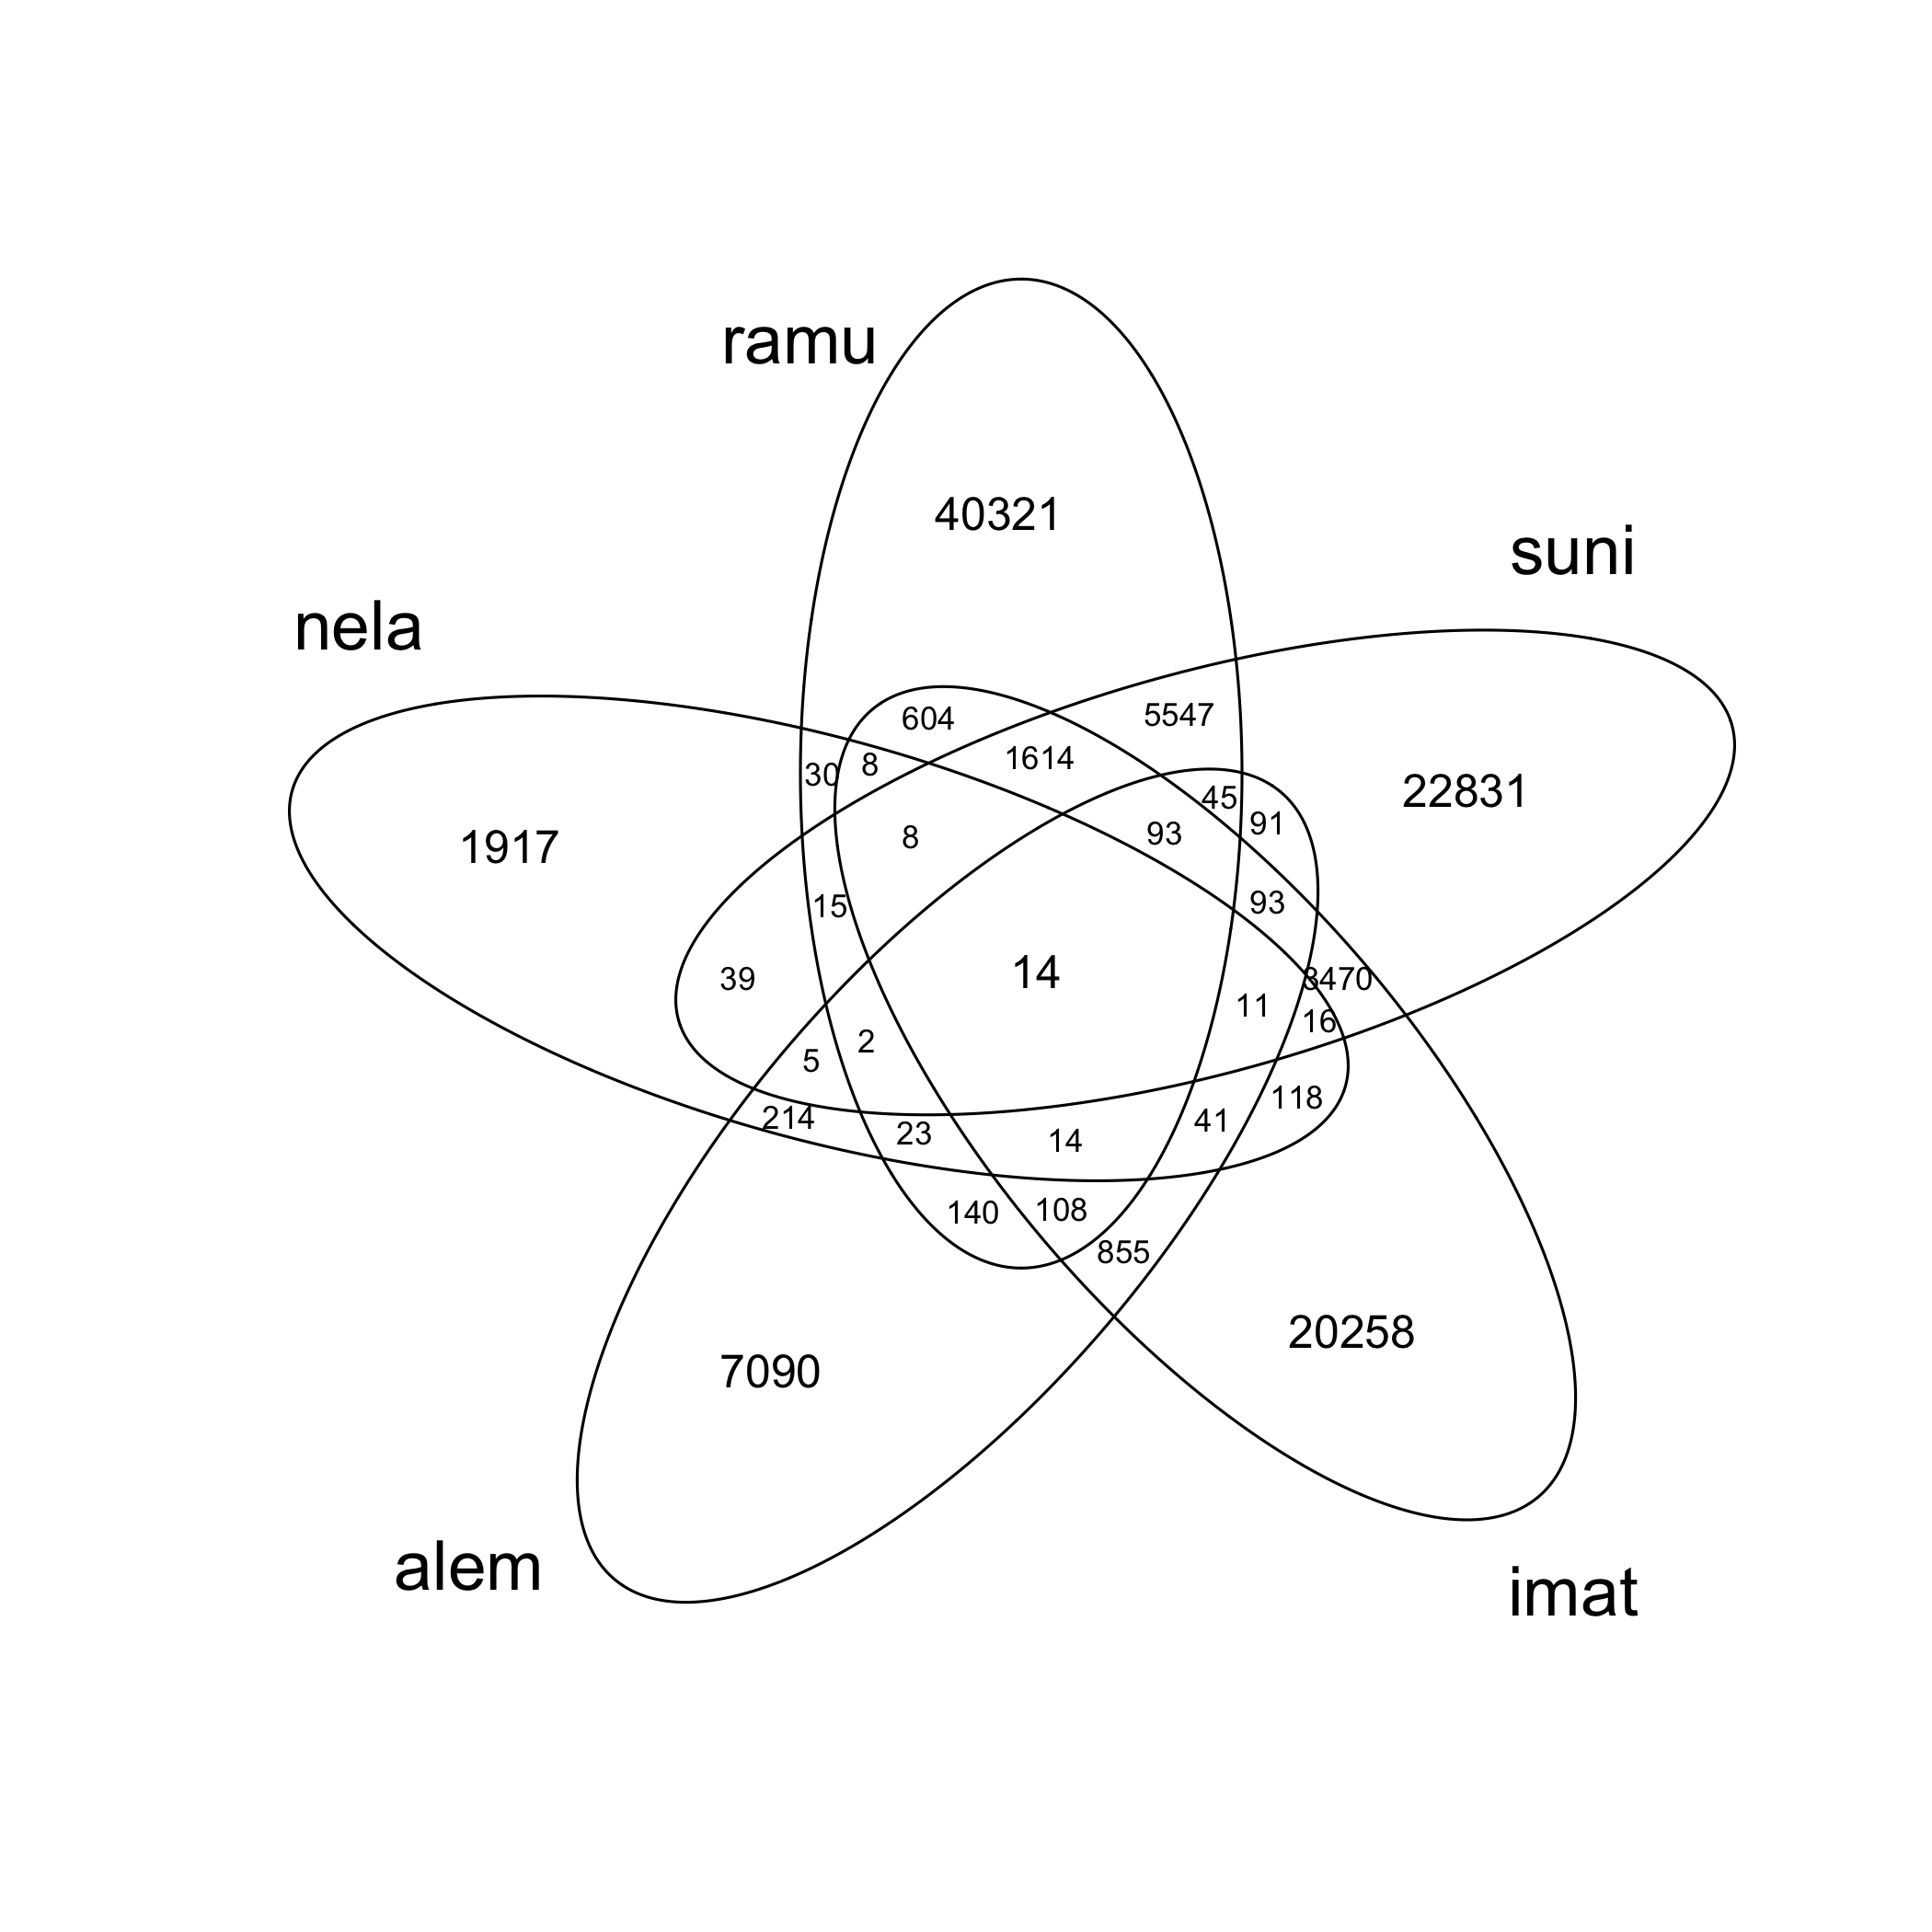
\includegraphics[width=.95\linewidth]{cited_sid.png}
  %\caption{}
  \label{fig:sub2}
\end{subfigure}
\caption{{\bf Intersecting Publications in Five Networks}  \emph{Left Panel.} Intersections were calculated across all five networks for citing\_pmids (the first generation of references) and displayed as a Venn diagram.
No publications are common to all five networks. A single publication is cited in four of five networks. \emph{Right Panel.} Intersections were calculated across all five networks for cited\_sids (the second generation of references) and displayed as a Venn diagram.
14  publications are common to all five networks. Abbreviations: alem (Alemtuzumab), imat (Imatinib), nela (Nelarabine), ramu (Ramucirumab), suni(Sunitinib)}
\label{fig:test}
\end{figure}

\begin{figure}[!h]
\centering
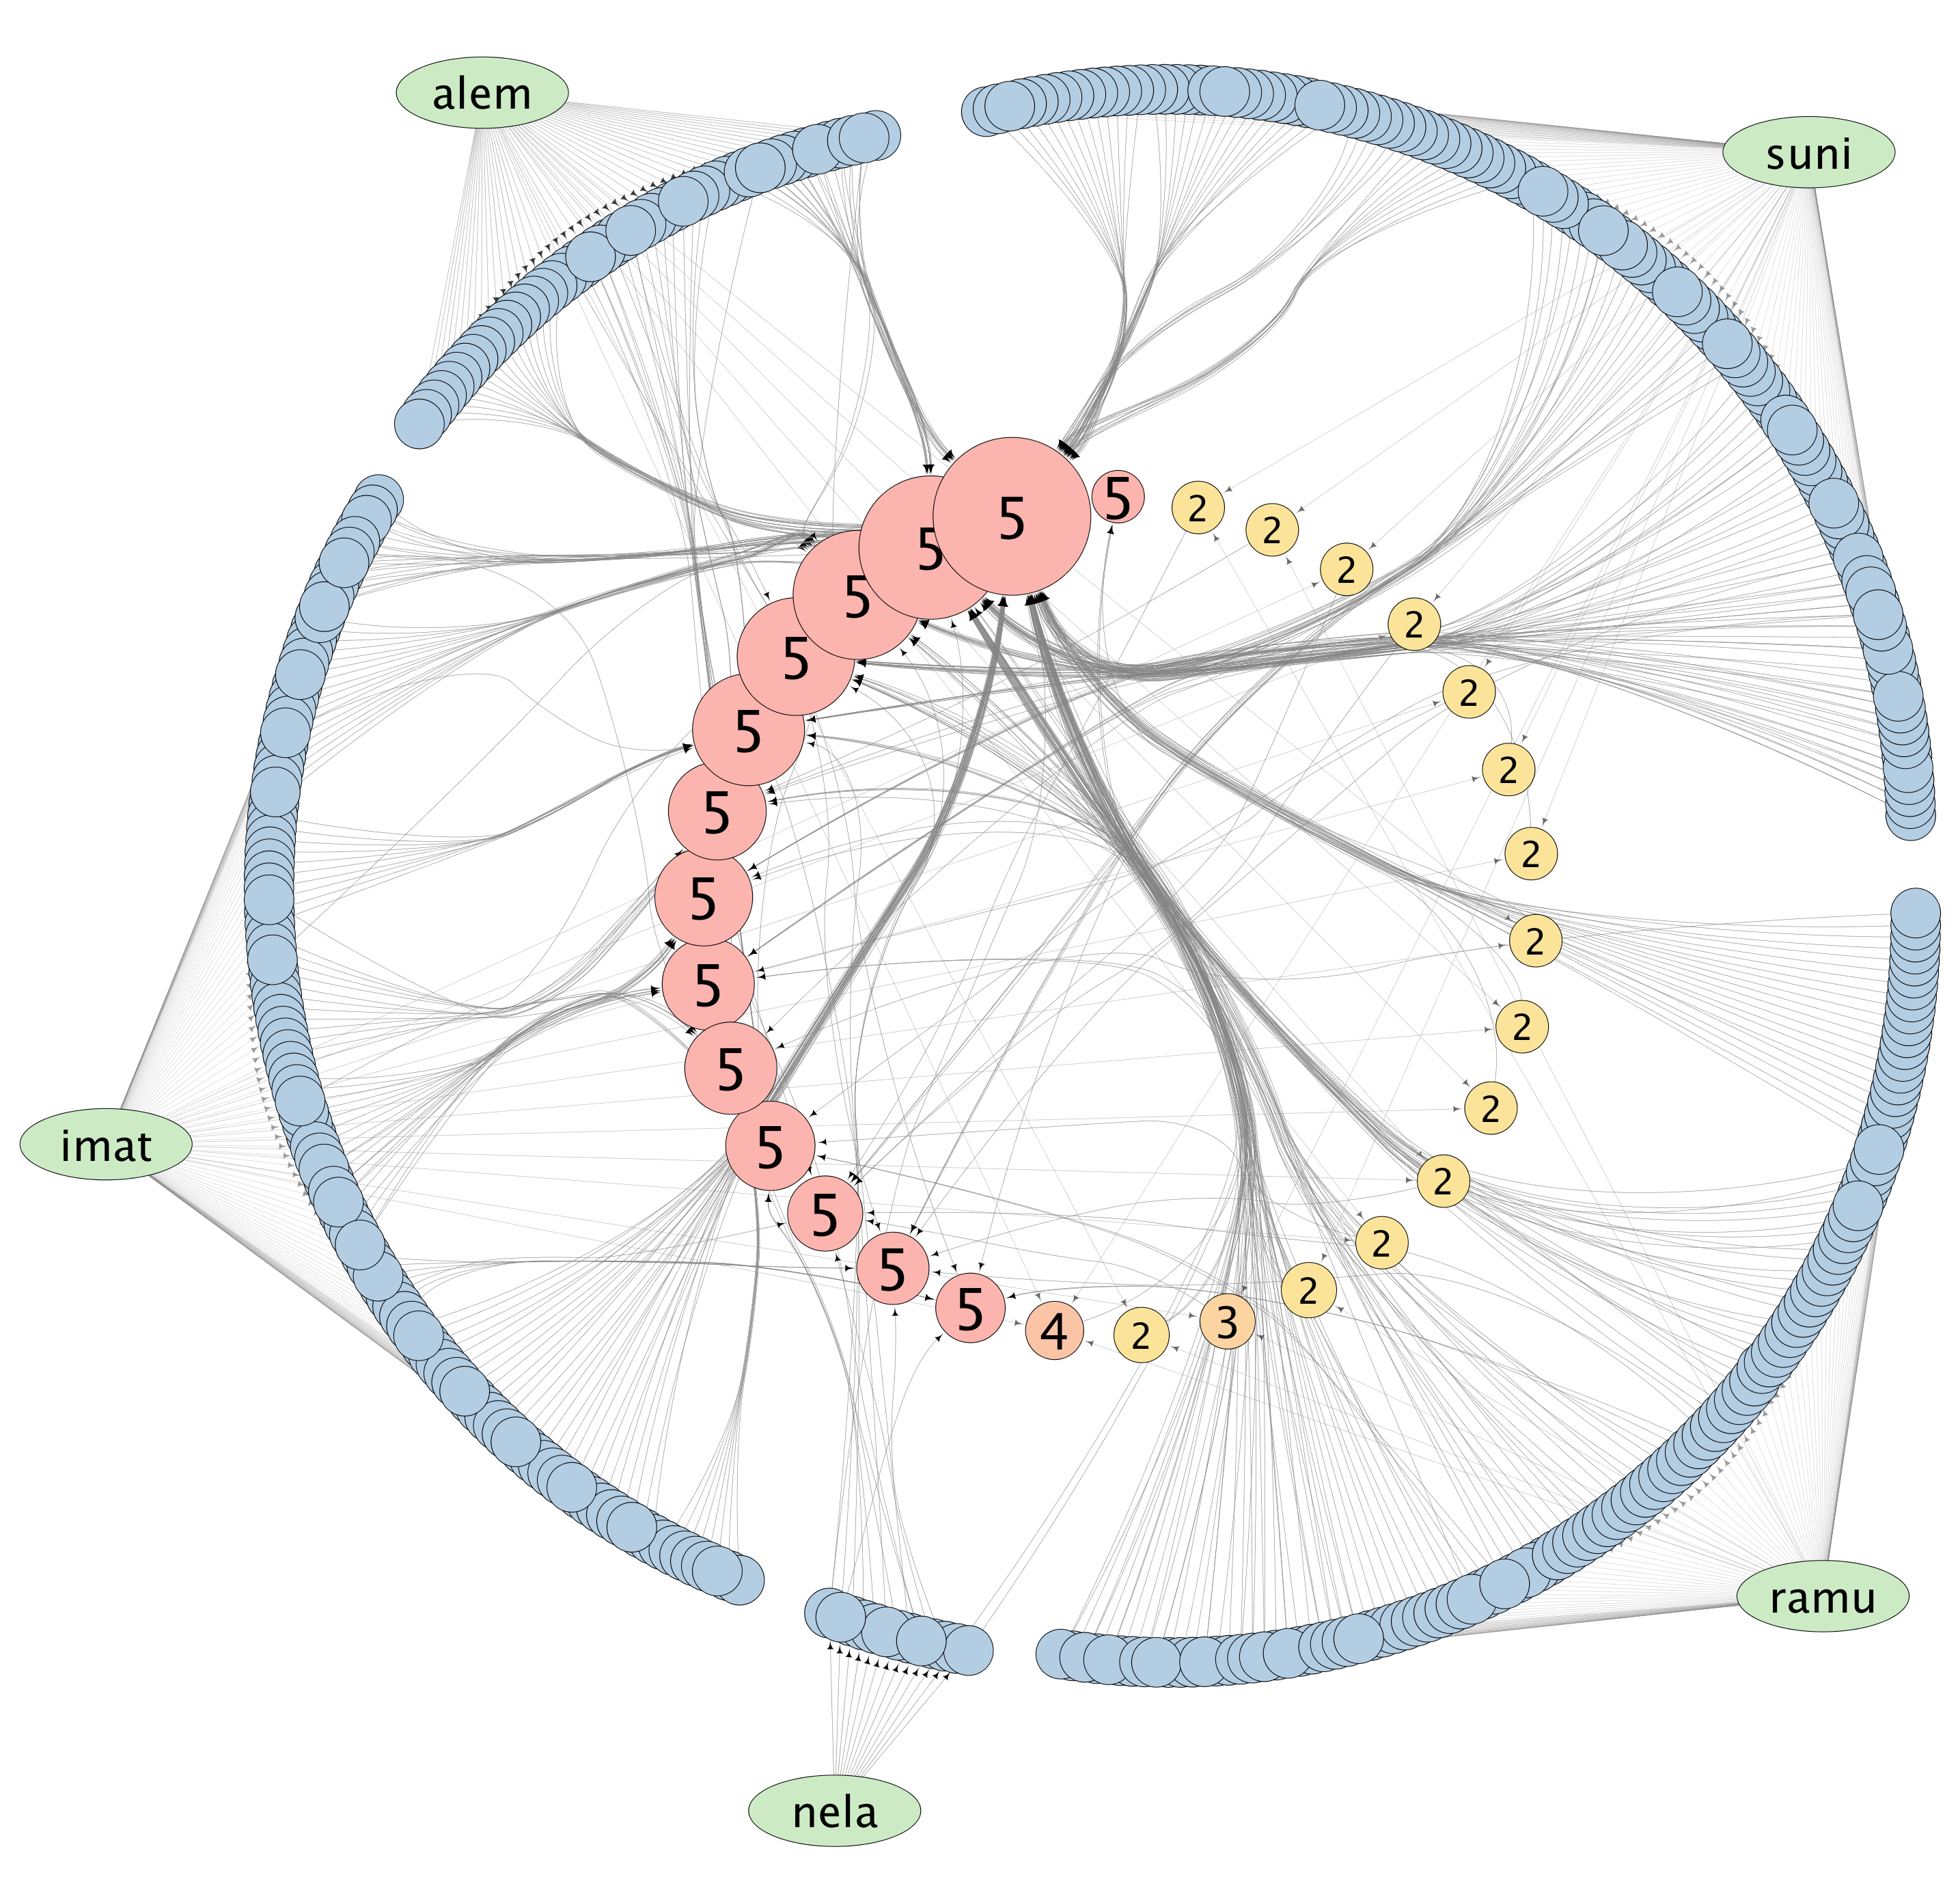
\includegraphics[scale=0.1]{cy_core14_v2csv_6b.png}
\caption{{\bf Core Publications in Networks}  The outer ring of blue nodes identifies first generation publications (citing\_sid) for each therapeutic. Nodes in the inner ring are sized by a gradient proportion to total degree count with an upper limit of 30 and are colored by a gradient proportional to the number of drug connections (2 to 5). 14  publications are common to all five networks (Table 3) and are colored red. The remaining nodes in the inner ring connect to between 2 and 4 drugs each and are labeled accordingly. Abbreviations: alem (Alemtuzumab), imat (Imatinib), nela (Nelarabine), ramu (Ramucirumab), suni(Sunitinib).}
\label{fig3}
\end{figure}
\clearpage

\begin{figure}[!h]
\centering
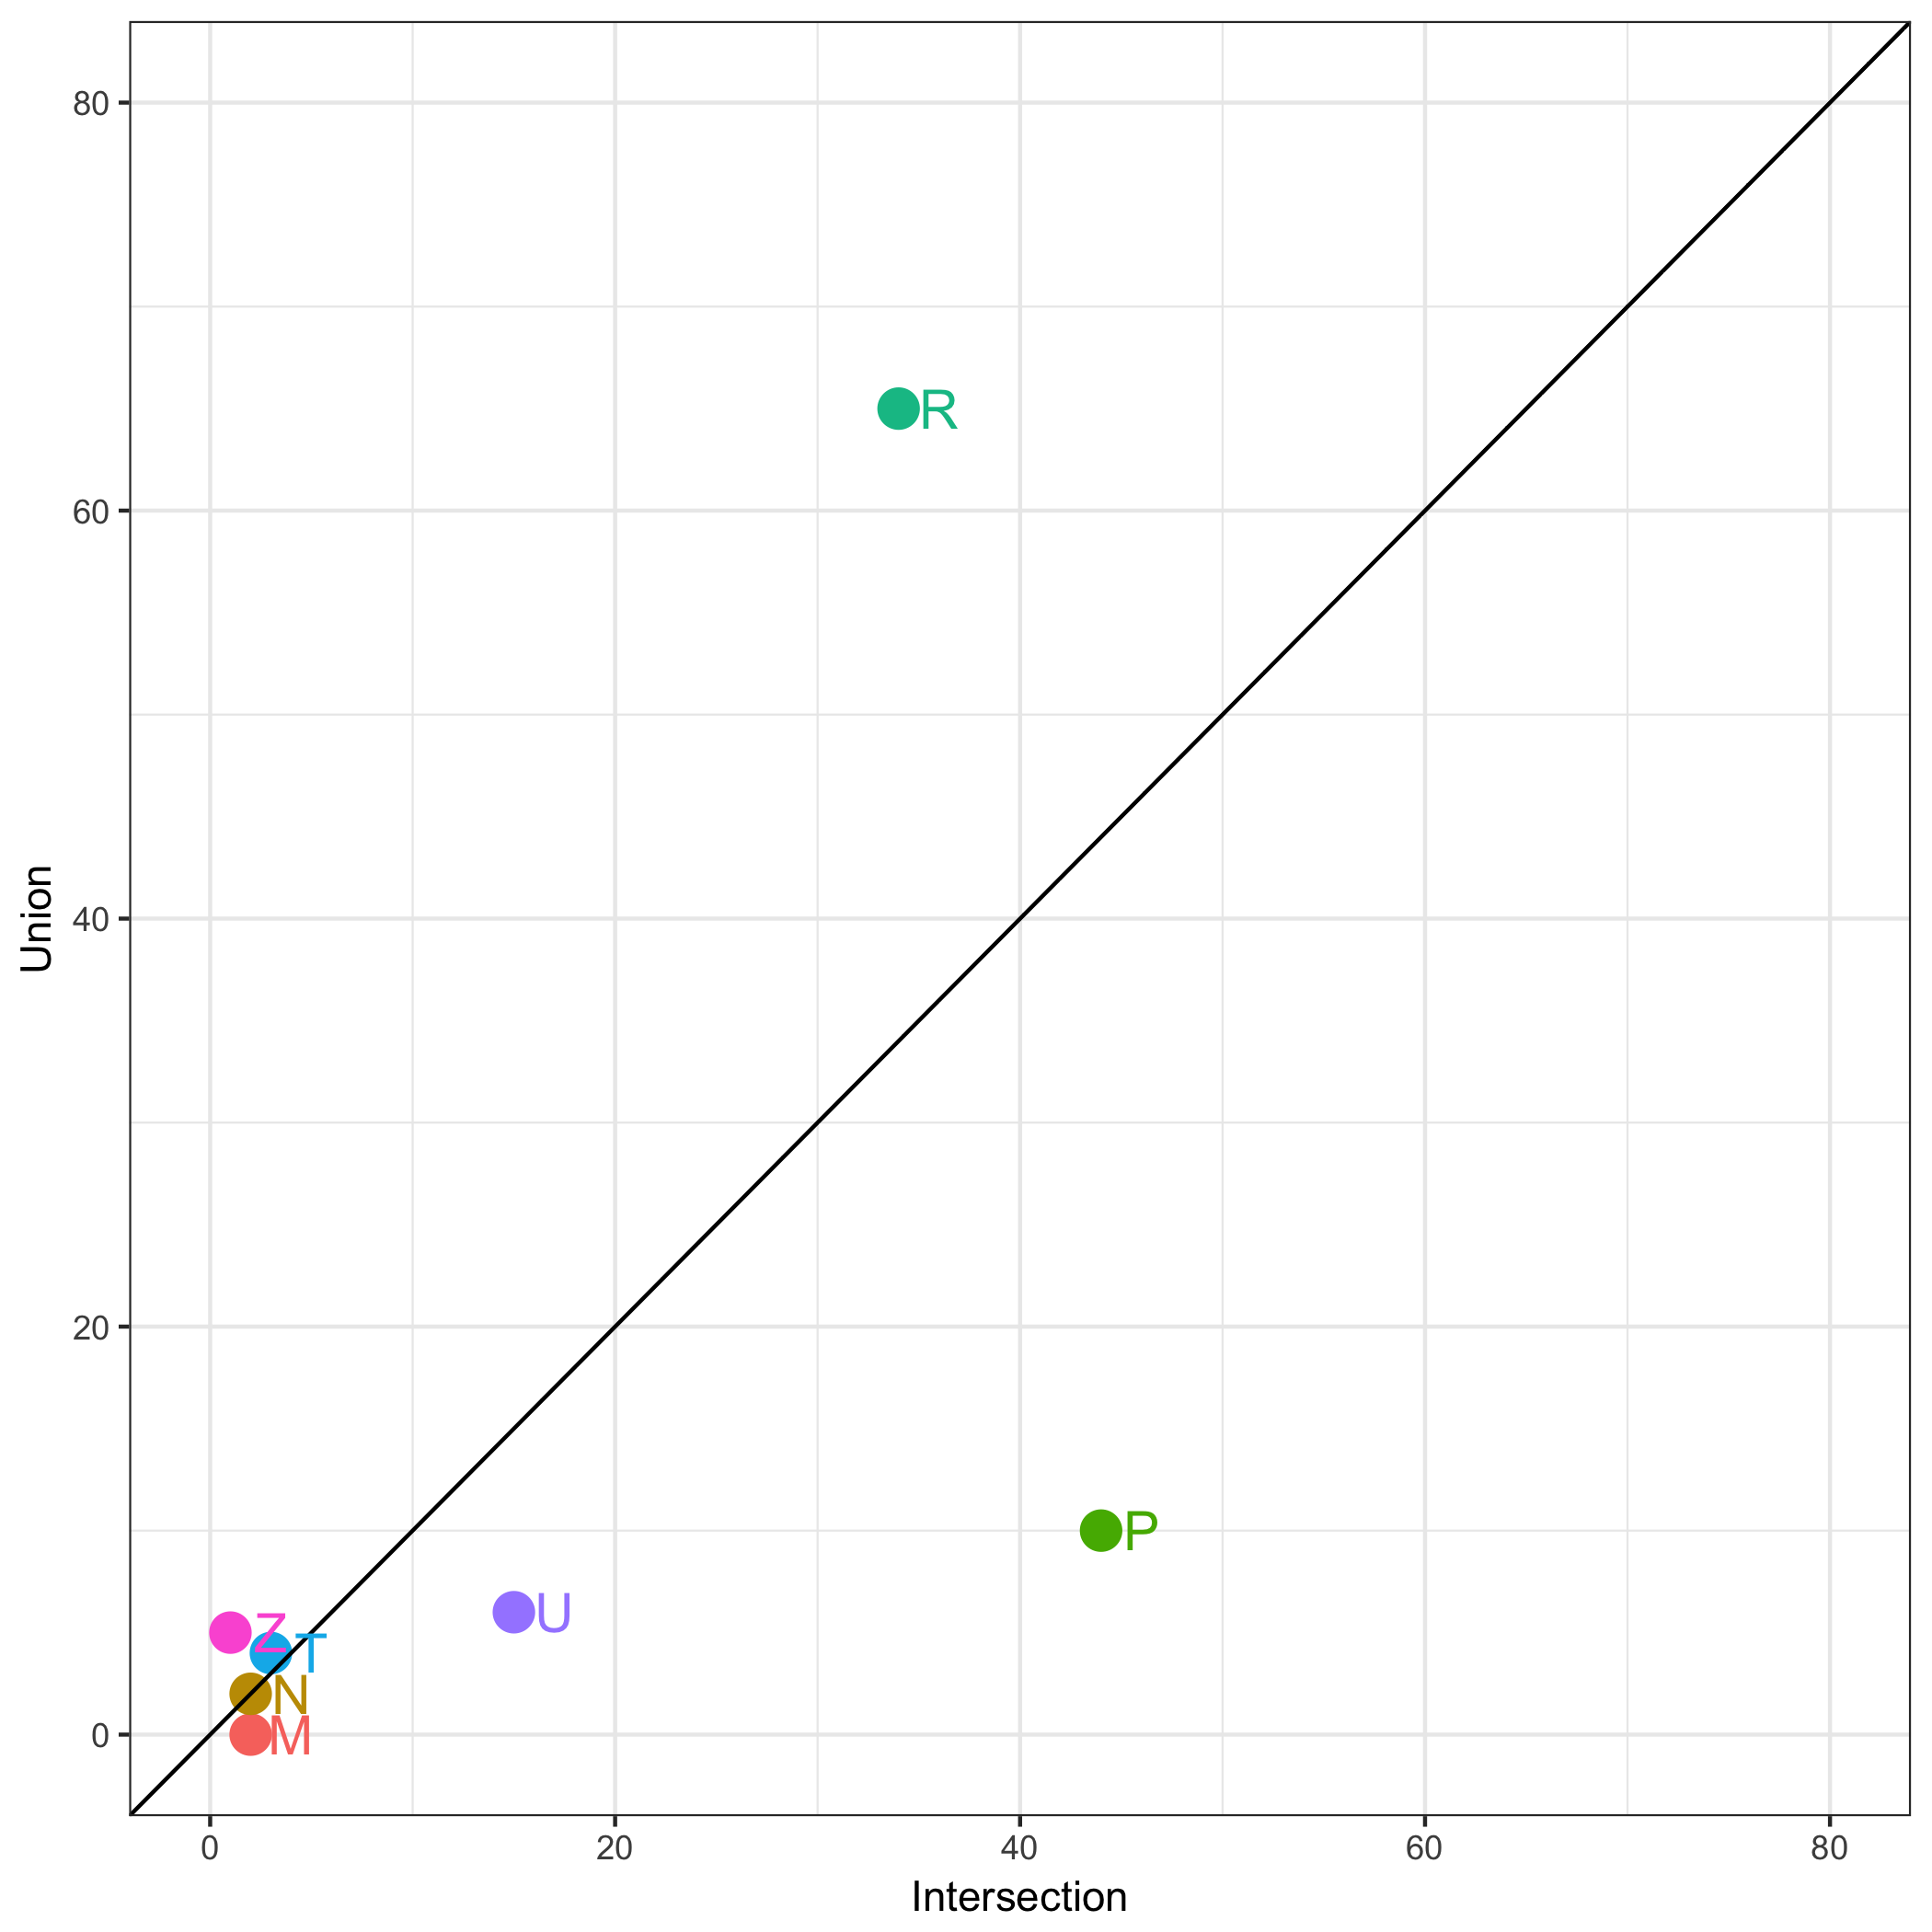
\includegraphics[scale=0.1]{proj_percent.png}
\caption{{\bf NIH Research Support} Grant and contract support for publications from NIH in the five networks was identified using ExPORTER data (Materials and Methods). 19,104 unique project numbers were identified of which 112 projects were common to all five networks. Projects were grouped by mechanism (i) P-  Research Program Projects and Centers (ii) R- Research Projects (iii) M-General Clinical Research Centers Programs (iv) N-Research and Development-Related Contracts (v) U-Cooperative Agreements (vi) T-Training Programs (vii) Z- Intramural Research. For each mechanism, the number of projects in the intersection of all five networks was plotted against the number in the union of all five networks (both expressed as percentages of their respective totals). A higher proportion of Research Program Projects and Centers awards is found in the intersection group.}
\label{fig4}
\end{figure}
\clearpage

\end{document}

